\documentclass[conference]{IEEEtran}
\IEEEoverridecommandlockouts
% The preceding line is only needed to identify funding in the first footnote. If that is unneeded, please comment it out.
\usepackage{cite}
\usepackage{amsmath,amssymb,amsfonts}
\usepackage{algorithmic}
\usepackage{graphicx}
\usepackage{textcomp}
\usepackage{xcolor}
\def\BibTeX{{\rm B\kern-.05em{\sc i\kern-.025em b}\kern-.08em
    T\kern-.1667em\lower.7ex\hbox{E}\kern-.125emX}}
    
\usepackage{listings}
\usepackage{xcolor}

\usepackage{hyperref}

%New colors defined below
\definecolor{codegreen}{rgb}{0,0.6,0}
\definecolor{codegray}{rgb}{0.5,0.5,0.5}
\definecolor{codepurple}{rgb}{0.58,0,0.82}
\definecolor{backcolour}{rgb}{0.95,0.95,0.92}

%Code listing style named "mystyle"
\lstdefinestyle{mystyle}{
  backgroundcolor=\color{backcolour},   commentstyle=\color{codegreen},
  keywordstyle=\color{magenta},
  numberstyle=\tiny\color{codegray},
  stringstyle=\color{codepurple},
  basicstyle=\ttfamily\footnotesize,
  breakatwhitespace=false,         
  breaklines=true,                 
  captionpos=b,                    
  keepspaces=true,                 
  numbers=left,                    
  numbersep=5pt,                  
  showspaces=false,                
  showstringspaces=false,
  showtabs=false,                  
  tabsize=2
}

%"mystyle" code listing set
\lstset{style=mystyle}
    
\begin{document}

\title{ECE 575 Final Project: Implementing a 5-stage processor pipeline in Python}

\author{\IEEEauthorblockN{Robert Werthman}
\IEEEauthorblockA{ECE 575 Section 02 \\
University of Michigan Dearborn}
}

\maketitle

\begin{abstract}
This document describes an implementation of a 5-stage instruction processing pipeline in the programming language python.  The processor, pipeline stages, instruction, and data memory can be represented in Python using object-oriented programming and python structures like lists and dictionaries.
\end{abstract}

\section{Introduction}
There are multiple ways to execute instructions in a processor.  One way is to execute one instruction in one clock cycle.  This is known as single cycle execution.  In single cycle execution the processor datapath which is defined as all the elements necessary to implement a set of instructions is designed such that all instructions that are part of the instruction set architecture are executed in a single cycle [2, p. 1].  An often used analogy to the execution of an instruction is doing laundry as mentioned in [1, p. 272].  Let's say the instruction you wanted to execute was to wash dirty cloths and put them away.  In a single cycle datapath the steps would be
\begin{enumerate}
    \item Put dirty cloths in washer.
    \item Once washer is done put dirty cloths in dryer.
    \item When dryer is done put clothes away
\end{enumerate}
As you can see each step depends on the completion of the previous step.  Imagine you had a roommate who also folded his/her clothes before putting them away was coming after you to do laundry.  The roommate has an additional step in their datapath and would have to wait for everything to be done before starting their load of laundry.  If you and your roommate were driven by a single clock cycle the cycle would have to last as long as the time to complete your roommate's clothes washing steps.  This is because in a single cycle datapath the cycle must last as long as the instruction that has the longest path to complete [1, p. 271].  It was determined this was not very efficient and a more efficient way of executing instructions was developed.  This better way to execute instructions in a processor called the pipelined datapath.

Think of an instruction as a series of steps.  All steps need to be completed in order for the instruction execution to be completed.  In a pipelined datapath one step of an instruction is executed every clock cycle instead of all of the steps of an instruction being executed every clock cycle.  Using the clothes washing analogy again, the steps in a pipelined datapath would be
\begin{enumerate}
    \item Put dirty cloths in washer.
    \item Once washer is done put dirty cloths in dryer.  Roommate puts dirty clothes in washer.
    \item Once dryer is done put clothes away.  Roommate puts clothes from washer into dryer.
    \item Roommate fold clothes.
    \item Roommate puts clothes away.
\end{enumerate}
You may have noticed the roommate does not have to wait for you clothes to be completely done.  The roommate can use the washer as long as you don't have any clothes in it.  This was found to be a more efficient datapath design for instructions than the single cycle datapath.
As noted in [1, pp. 286] the steps of an instruction in a pipelined datapath are made into 5-stages
\begin{enumerate}
\item IF: Instruction fetch
\item ID: Instruction decode and register file read
\item EX: Execution or address calculation
\item MEM: Data memory access
\item WB: Write Back
\end{enumerate}
This stages can be modelled in Python as objects connected to each other.  The rest of this document describes the implementation of this modelling.


\section{Architecture}

\begin{figure}
    \centering
    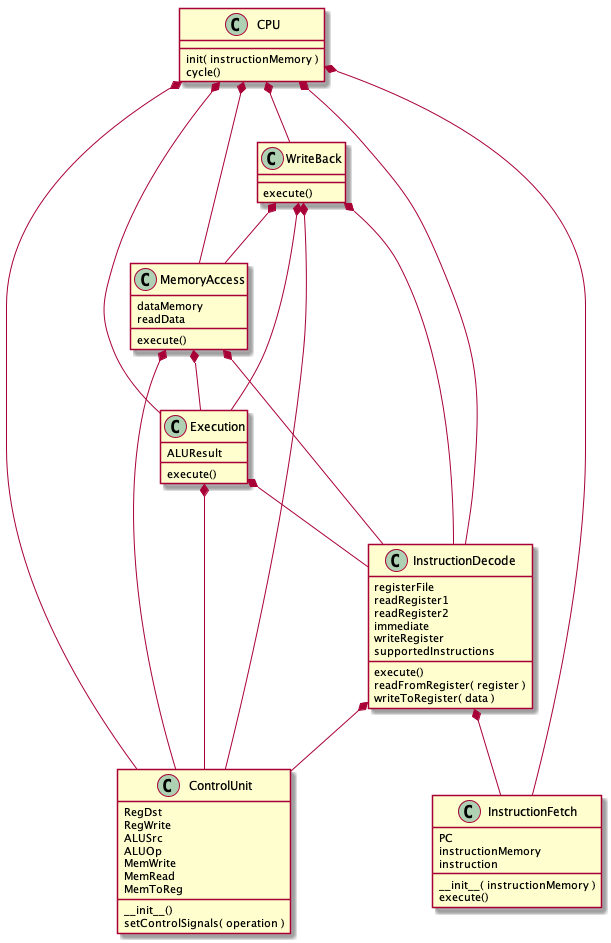
\includegraphics[scale=.4]{architecture.png}
    \caption{Class Diagram of Python Implementation}
    \label{fig:class_diagram}
\end{figure}

The Python implementation is made of the 5 pipeline stages mentioned in the introduction.  These are represented as Python classes.  Each of these stages consist of additional components.
\begin{itemize}
    \item instruction memory
    \item data memory
    \item a register file
    \item an ALU (arithmetic logic unit)
    \item a PC (program counter)
    \item a control unit
\end{itemize}
All of these components belong to different stages of the pipeline except for the control unit which is used in almost all stages of the pipeline.  A class diagram of the architecture can be seen in figure \ref{fig:class_diagram}.

\subsection{IF: Instruction Fetch}

\begin{figure}
    \centering
    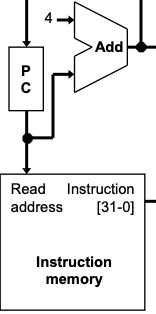
\includegraphics[scale=.4]{instructionfetch.png}
    \caption{Instruction Fetch Stage [2]}
    \label{fig:instructionfetch}
\end{figure}

The instruction fetch part of the pipeline takes the program counter (PC) and fetches the instruction at the address of the program counter [1, pp. 300].  It increments the program counter to the next address.  These things are done in a class method called execute which is pipeline stage contains

\subsubsection{Instruction Memory}

Instruction memory is represented as a Python list that is passed into the instruction fetch class at initialization.  Each instruction itself is also a Python list.  Depending on the instruction type the list is made up of the opcode, source and destination registers, address/immediate, etc.  An example of an add instruction in python 

\begin{lstlisting}[language=Python]
# An add instruction
instruction = [ "add", "r1", "r2", "r3" ]
\end{lstlisting}

which means [3, pp. 194]

\begin{center}
\begin{tabular}{|c|c|c|c|}
\hline
     op & rs & rt & rd \\
\hline
\end{tabular}
\end{center}

To access an instruction memory you use an index in the list.  For example
\begin{lstlisting}[language=Python]
# Get the first instruction from instruction memory
instruction = instructionMemory[0]
\end{lstlisting}

\subsubsection{Program Counter}

The program counter is a python variable that is initialized as 0 and is increment by 1 for every call to execute method of the instruction fetch class.

\subsection{ID: Instruction Decode}

\begin{figure}
    \centering
    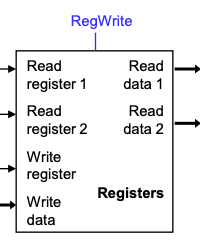
\includegraphics[scale=.4]{instructiondecode.png}
    \caption{Instruction Decode Stage [2]}
    \label{fig:instructiondecode}
\end{figure}

In the instruction decode stage of the pipeline the control signals are set in the control unit based on the opcode in the instruction.  The instruction is referenced from the instruction fetch class through a member variable.  The read registers, rs and rt, are stored in the class as well as the write register, and the immediate/address value if one exists.  These come from the instruction from the instruction fetch stage.  Only add, load word (lw), and store word (sw) are supported instructions at this time.  The supported instructions are mapped to their instruction type in a dictionary.

\begin{lstlisting}[language=Python]
self.supportedInstrutions = {
            "add" : "rtype",
            "lw"  : "itype",
            "sw"  : "itype"
        }
\end{lstlisting}

The instruction type is used to determine if there will be an immediate/address in the instruction or not.  There are 2 methods that are a part of this stage.  They are the readFromRegister and writeToRegister methods simliar to the read data and write data in [1, pp. 301].
The instruction decode stage has a register file.

\subsubsection{Register File}

The register file is a dictionary with the register has the key and value of the register as the value.
\begin{lstlisting}[language=Python]
self.registerFile = {
            "r1" : 2,
            "r2" : 1,
            "r3" : 0
        }
\end{lstlisting}
Only 3 registers are supported at this time.

\subsubsection{Control Unit}

\begin{figure}
    \centering
    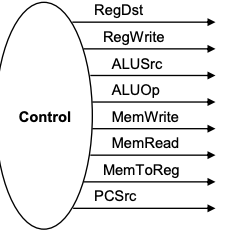
\includegraphics[scale=.4]{controlunit.png}
    \caption{Datapath Control Unit}
    \label{fig:controlunit}
\end{figure}

The control unit is a class that contains just member variables which are the control signals to the pipeline.  The signals are set to their values depending on what the opcode of the instruction is.  The control unit is seen in figure \ref{fig:controlunit}

\subsection{EX: Execution}

\begin{figure}
    \centering
    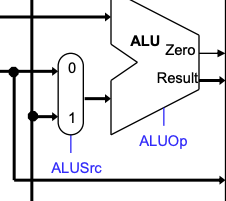
\includegraphics[scale=.4]{execution.png}
    \caption{Execution Stage}
    \label{fig:execution}
\end{figure}

In the execution state of the pipeline we compute the result of arithmetic between 2 registers, or compute an address to load or store a value in data memory.  The execution stage depends on control signal ALUOp to tell it was arithmetic operation to perform.  It also depends on ALUSrc to tell it what should be the source of the second operand.  The execution statge is figure \ref{fig:execution}  Right now only add is supported but this still allows for an add r-type instruction or the load word or store word i-type instructions.

The result of the arithmetic operation is stored as a class instance member variable that both the Memory Access and Write Back stages will use.

\subsection{MEM: Memory Access}

In the memory access stage you can read or write data to data memory or not do anything if the instruction is an r-type instruction.  This stage is comprised of the data memory and the ability to used an address to read and write data to.

\subsubsection{Data Memory}

\begin{figure}
    \centering
    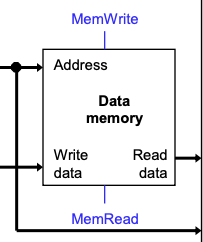
\includegraphics[scale=.4]{memoryaccess.png}
    \caption{Memory Access Stage [2]}
    \label{fig:memoryaccess}
\end{figure}

Much like the instruction memory, data memory is represented as a list of integers.

\begin{lstlisting}[language=Python]
# Data memory
dataMemory = [1, 2, 3, 4]
\end{lstlisting}

The ALUResult that comes from the Execution stage is used as an index into the data memory list.  Depending on the values of the control signals MemRead or MemWrite you will be either reading or writing to the data memory.  An if/else statement is used with control signals as the conditions to read or write to data memory.

\subsection{WB: Write Back}

\begin{figure}
    \centering
    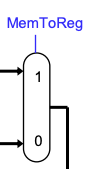
\includegraphics[scale=.4]{writeback.png}
    \caption{Write Back Stage [2]}
    \label{fig:writeback}
\end{figure}

The Write Back is the simplest of all of the stage but it is the stage that depends on the most previous stages.  As depicted in [1, pp. 301] this stage has a MUX that is controlled by the MemToReg control signal.  The value of this signal depends on the instruction being executed.  The MUX is represented by an if/else statement with the MemToReg as the if condition.

\begin{lstlisting}[language=Python]
if controlUnit.MemToReg:
    ID.writeToRegister( MEM.readData )
else:
    ID.writeToRegister( EX.ALUResult )
\end{lstlisting}

\subsection{CPU}
The CPU is the main class that creates and contains all of the pipeline stages.  It is the class that contains the initialization of the instruction memory, passes it to the instruction fetch stage, and starts the execution of the pipeline.

The the execution of the stages is done in a method called \textit{cycle}.  For each instruction in instruction memory execute the pipeline stages in order.

\begin{lstlisting}[language=Python]
for instruction in instructionMemory:
    IF.execute()
    ID.execute()
    EX.execute()
    MEM.execute()
    WB.execute()
\end{lstlisting}

\section{Testing and Verification}
Test driven development was used when developing this project.  This means tests were written, the tests failed, and then code was written to make the tests pass.  For each class a python file containing containing tests was created.  These tests were used to verify the behavior of each of the methods of the class.
The main integration driver were the tests for the CPU.  In those tests I would create a CPU that contained all of the stages, create an instruction memory with one instruction, and have the CPU process the instruction through all of the stages.  At the end I would check to see if a register has the expected value or if the data memory was written in the right location with the expected value 

\section{Open Issues And Future Work}

\begin{thebibliography}{00}
\bibitem{b1} J. Hennessy and D. Patterson, \textit{Computer Organization And Design: The Hardware/Software Interface}, 5th ed. Waltham, MA: Elsevier, 2014.
\bibitem{b2} L. Ceze, "A single-cycle MIPS processor". University of Washington, Computer Science and Engineering, CSE 378, Winter 2009. [Online]. Available: \url{https://courses.cs.washington.edu/courses/cse378/09wi/lectures/lec07.pdf}. [Accessed December 03, 2019]
\bibitem{b3} P. Gillard, "The MIPS instruction set architecture". Memorial University, Department of Computer Science, CS 3725. [Online]. Available: \url{http://web.cs.mun.ca/~paul/cs3725/material/review.pdf}. [Accessed December 03, 2019]
\end{thebibliography}

\end{document}
